\chapter{让圆盘运动：位置、速度与力}\label{ch:robot}
\begin{notebox}
\textbf{目标}\quad 区分理想位置执行与物理运动；让碰撞半径真正约束移动。\\
\textbf{先修}\quad 前三章、速度与加速度的含义。先运行，再推导。
\end{notebox}

\section{圆心状态与圆盘外形}
机器人用圆心描述状态，圆盘描述占据的空间：
\begin{equation}
x=(p,v,\psi,\omega),\qquad
p=(p_x,p_y),\quad v=(v_x,v_y).
\end{equation}
位置单位 m，速度 m/s，yaw 为 rad，角速度 rad/s。位置和速度在 odom 系表达；
本章的 map 与 odom 重合。半径 r 单独参与碰撞，不把“质点状态”误解为“没有体积”。
若 r=0，才是几何质点；屏幕上的小点仅用于看清位置。

控制量不同，模型的物理意义就不同。理想到点输入目标位姿；速度模型输入平面速度；
惯性模型输入力和偏航力矩。它们分别使用不同话题，不能把同一个数值悄悄解释成另一种单位。
先完成最容易运行的理想到点，再逐项加入连续运动模型。

\section{先让机器人到一个点}
停止之前的场景，重新构建并加载 install 后运行：
\begin{lstlisting}[language=bash,numbers=none]
ros2 launch motion2d_bringup ch04.launch.py model:=ideal
\end{lstlisting}
在 RViz2 用 2D Goal Pose 工具点击、拖动，指定目标位置和 yaw。工具向
\code{/command/pose} 发布消息。也可在第二个已加载 ROS 环境的终端发送：
\begin{lstlisting}[language=bash,numbers=none]
ros2 topic pub --once /command/pose geometry_msgs/msg/PoseStamped \
  "{header: {frame_id: odom}, pose: {position: {x: -7.0, y: -8.0}, orientation: {w: 1.0}}}"
\end{lstlisting}
默认从 $(-8,-8)$ 移到 $(-7,-8)$，图中留下接受过的运动轨迹。目标在下一 tick 才执行；
暂停时发目标，圆盘保持不动，单步后才到达目标。

\clearpage
\section{扫过的空间也要安全}
起终点安全并不足够。半径 r 的圆盘沿线段 $[p_0,p_1]$ 移动，扫过的区域是胶囊形。
对于圆心 c、半径 R 的障碍，无碰撞要求
\begin{equation}
\operatorname{dist}(c,[p_0,p_1])>R+r.
\end{equation}
这里直接复用第 03 章的点线段距离。对凸多边形，检查起终点和运动线段到每条边的距离；
对矩形边界，内缩后的矩形是凸集，检查两个端点即可保证整条直线留在其中。

\begin{center}
\begin{tikzpicture}[x=1cm,y=1cm]
\fill[tealblue!12,rounded corners=8mm] (-3,-.45) rectangle (3,.45);
\draw[tealblue,dashed,rounded corners=8mm] (-3,-.45) rectangle (3,.45);
\draw[-{Stealth},thick,navy] (-2.55,0) -- (2.55,0);
\draw[fill=white,tealblue,thick] (-2.55,0) circle (.45);
\draw[fill=white,tealblue,thick] (2.55,0) circle (.45);
\draw[fill=muted!50,navy] (0,.15) circle (.55);
\node[below] at (-2.55,-.5) {$p_0$};
\node[below] at (2.55,-.5) {$p_1$};
\node[above] at (0,.8) {端点自由，整段被挡住};
\end{tikzpicture}
\end{center}

\par\noindent\begin{minipage}{\linewidth}
\lstinputlisting[language=C++,linerange={sweep_begin-sweep_end},
  includerangemarker=false]{../ros2_ws/src/motion2d/src/sim/swept_collision.cpp}
\end{minipage}\par
代码没有按固定间距抽样，因此不会因为障碍很薄、目标很远，就从障碍另一侧“穿过去”。
这是连续直线扫掠的几何检查，浮点实现仍受数值精度限制。

\clearpage
\section{理想到点不产生真实 IMU}
通过几何检查后，理想模型直接赋值目标位姿：
\par\noindent\begin{minipage}{\linewidth}
\lstinputlisting[language=C++,linerange={ideal_begin-ideal_end},
  includerangemarker=false]{../ros2_ws/src/motion2d/src/sim/ideal_model.cpp}
\end{minipage}\par
位置在一个 tick 中改变，不代表机器人以一个有限速度完成了运动。速度和加速度字段为
未使用的零值；不能对这种跳变做差分，再把结果称为模拟 IMU。平滑轨迹执行将在轨迹章节加入。

\begin{figure}[ht]
\centering
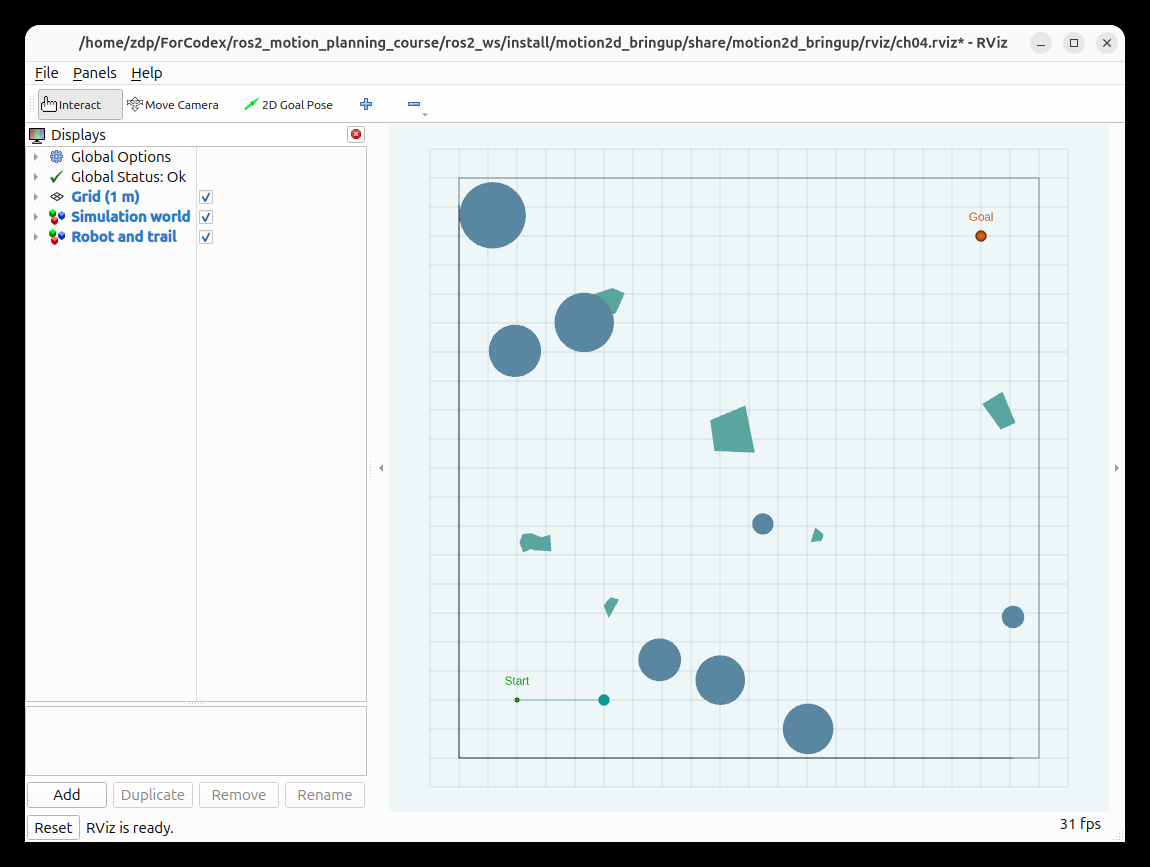
\includegraphics[width=.78\linewidth]{figures/ch04_ideal_rviz.png}
\caption{实际 RViz2 画面：世界、圆盘与已接受的移动轨迹。}
\end{figure}

\section{冻结试验与重新开始}
若扫掠检查失败，程序不接受候选状态：位置、速度和时间停在上一个通过检查的 tick，
\code{/sim/status} 为 \code{collision_predicted}，圆盘变红。
这是提前终止试验，尚未模拟接触力、反弹或摩擦。它没有把撞入障碍的状态推回自由空间。
需要调用 reset 才能继续。

\begin{lstlisting}[language=bash,numbers=none]
ros2 service call /sim/reset std_srvs/srv/Trigger "{}"
ros2 service call /sim/step std_srvs/srv/Trigger "{}"
ros2 service call /sim/pause std_srvs/srv/SetBool "{data: false}"
\end{lstlisting}
reset 开始新试验：回初始状态、清空待执行命令与轨迹、仿真时间归零并暂停。
单步推进一个 dt；恢复运行不改变 dt。墙钟定时器决定运行快慢，整数 tick 决定模拟时间。

% extension_sections
\clearpage
\section{接口、练习与验收}
本章默认 dt=0.005 s。位姿输入接受 odom/map；map 可用是因为本章二者重合。
姿态必须是平面单位四元数，不能把四个分量全填零。时间戳为零表示下一 tick；
非零时间戳只接受当前模拟时刻附近的命令，过旧或过远的未来命令被拒绝。

\code{/sim/pose}、\code{/sim/velocity}、\code{/sim/acceleration} 都是真值调试输出，
平移分量在 odom 系。第 07 章才引入规范的里程计消息与选源，
后续 SLAM 不得读取这些调试话题。本章没有激光或 IMU。

\begin{enumerate}
\item \textbf{理解：}给一个起终点都自由但中间碰撞的例子。为什么瞬时位置赋值不适合 IMU？
\item \textbf{代码 ch04-1：}完成 \path{exercises/ch04/starter/sweep_circle.hpp}。
复用点线段距离，判定圆盘与圆障碍的整段扫掠；相切必须判为碰撞。
\item \textbf{实验：}暂停后发目标并单步；改变半径重复同一条贴近障碍的移动。
记录 seed、半径、起终点和结果。不要把显示尺寸当作碰撞半径。
\end{enumerate}

从仓库根目录编译练习：
\begin{lstlisting}[language=bash,numbers=none]
g++ -std=c++17 -I/usr/include/eigen3 \
  -Iros2_ws/src/motion2d/include -Iexercises/ch04/starter \
  exercises/ch04/check_sweep.cpp \
  ros2_ws/src/motion2d/src/geometry/obstacles.cpp \
  -o /tmp/ch04_sweep
/tmp/ch04_sweep
\end{lstlisting}
提示和参考解分开存放；将 starter 替换为 solutions 可以验证参考解。
演示运行时，从工作空间执行：
\begin{lstlisting}[language=bash,numbers=none]
/usr/bin/python3 ../scripts/check_ch04.py
\end{lstlisting}
脚本会改变场景状态，检查暂停命令、单步、错误帧、碰撞冻结与 reset。
算法测试另外覆盖薄墙和零半径质点。

\begin{notebox}
\textbf{没有移动时先检查}\quad 是否暂停、是否需要 reset、模型是否与输入话题对应，
再检查 frame 和四元数。只运行一个课程 launch，避免多个时钟或 TF 发布者。
\end{notebox}
